\section{Advanced Classification}
\label{sec:advanced_classification}

In this section, classification results are showcased for two
target variables: \texttt{averageRating} (properly binned into
6 classes), and \texttt{titleType} (with 6 classes).

\textcolor{red}{We then applied multiple classification models using the data as preprocessed previously (see Section~\ref{sec:understanding_preparation}).}   
\textcolor{blue}{The first target variable is \texttt{titleType}, which includes six categories: 
\textit{movie}, \textit{short}, \textit{tvEpisode}, \textit{tvSeries}, 
\textit{tvSpecial}, and \textit{video}. 
The classes are not equally distributed, with \textit{tvSpecial} and \textit{video} 
being significantly under-represented compared to the others. Entries labeled as \textit{videoGame} were removed from both the training and testing sets, 
as they were too few to be useful for classification. 
The remaining categories were merged into broader groups according to the following mapping: 
\textit{movie} and \textit{tvMovie} were grouped as \textit{movie}, 
\textit{short} and \textit{tvShort} were grouped as \textit{short}, 
\textit{tvSeries} and \textit{tvMiniSeries} were grouped as \textit{tvSeries}, 
while \textit{tvEpisode}, \textit{tvSpecial} and \textit{video} were left unchanged. 
All feature columns were standardized using a \textit{StandardScaler}. 
In addition, the variable \texttt{canHaveEpisodes} was removed prior to training, 
since it provides direct information about the target \texttt{titleType} 
and could therefore introduce data leakage.}
%-------------------------------------------------------------------------------

\subsection{Logistic Regression}
\label{subsec:logistic}

%-------------------------------------------------------------------------------
% titleType logistic
%-------------------------------------------------------------------------------
For the classification of the \texttt{titleType} variable, the target was transformed 
into numerical labels using \textit{LabelEncoder} and all numerical features were scaled 
with \texttt{StandardScaler} to ensure comparability across variables.

Since the problem is multi-class, we chose to present the results using the 
\textit{One-vs-Rest (OVR)} approach, which trains a binary classifier for each class. 
We also tested the \textit{multinomial} strategy, but it was significantly slower and 
produced comparable results, so OVR was selected for efficiency.

To optimize the model, a hyperparameter search was performed using 
\texttt{RandomizedSearchCV} with \texttt{StratifiedKFold} (5 folds), ensuring that the class 
distribution was preserved in each fold. The solver was set to \texttt{saga}, and the 
parameters tested included the regularization term $C$ (50 values logarithmically spaced 
between $10^{-3}$ and $10^2$), \texttt{penalty} (\texttt{l2} and \texttt{l1}), and 
\texttt{class\_weight} (\texttt{None} and \texttt{balanced}). The hyperparameter 
search was performed using \texttt{f1\_macro} as the scoring metric to balance 
performance across all classes. The best parameters selected by the search were 
\textbf{C = 2.95}, \textbf{penalty = l1}, and \textbf{class\_weight = balanced}.

For computational efficiency, the search was conducted on a 10\% stratified sample 
of the dataset, which was approximately representative of the original class distribution. The final 
model was then refitted on the full dataset using the best parameters. Evaluation on 
the test set was carried out using the confusion matrix, classification report, and 
one-vs-rest ROC curves for each class. The main performance metrics are summarized in 
Table~\ref{tab:logistic_report_t}, and the corresponding ROC curves are shown in 
Figure~\ref{fig:log_roc_curves_t}. 

\begin{figure}[ht]
    \centering
    \begin{minipage}{0.45\textwidth} 
    \centering
    \captionof{table}{Classification report for \texttt{titleType}}
    \label{tab:logistic_report_t}
    \small 
    \begin{tabular}{lccc}
    \hline
    \textbf{Class} & \textbf{Precision} & \textbf{Recall} & \textbf{F1-score}\\
    \hline
    tvEpisode  & 0.90 & 0.88 & 0.89  \\
    movie      & 0.92 & 0.65 & 0.76  \\
    short      & 0.74 & 0.87 & 0.80  \\
    tvSeries   & 0.50 & 0.35 & 0.41  \\
    video      & 0.21 & 0.47 & 0.29  \\
    tvSpecial  & 0.07 & 0.52 & 0.12  \\
    \hline
    \textbf{Accuracy}    & \multicolumn{3}{c}{0.75} \\
    \textbf{Macro avg}   & 0.56 & 0.62 & 0.54  \\
    \textbf{Weighted avg}& 0.83 & 0.75 & 0.78  \\
    \hline
    \end{tabular}
    \end{minipage}
    \hfill
    \begin{minipage}{0.4\textwidth} 
    \centering
    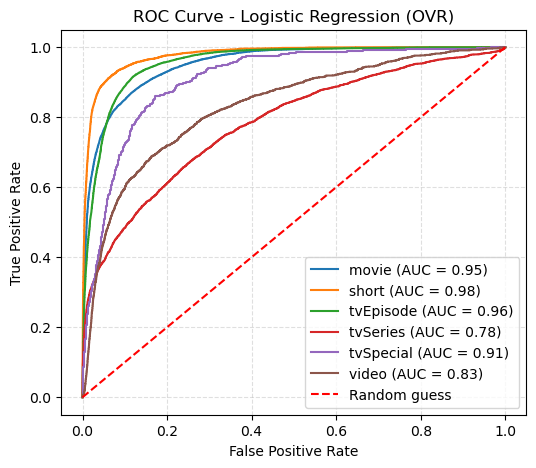
\includegraphics[width=\textwidth]{plotsss/log_roc_curves_t.png} 
    \captionof{figure}{ROC Logistic Regression}
    \label{fig:log_roc_curves_t} 
    \end{minipage}
    \end{figure}


From the results, we observe that the model achieves high performance for the 
\texttt{movie}, \texttt{short}, and \texttt{tvEpisode} classes, with F1-scores of 0.76, 
0.80, and 0.89, respectively. The model performs less well on \texttt{tvSeries}, 
\texttt{tvSpecial}, and \texttt{video}, likely due to lower support in the dataset.
Overall, the model reaches an accuracy of 0.75, 
a macro-average F1 of 0.54, and a weighted F1 of 0.78. These results highlight that 
while the model discriminates well among the more common classes, its performance is still
limited for rarer classes. 
This pattern is also reflected in the ROC curves shown in Figure~\ref{fig:log_roc_curves_t}, 
where the model clearly separates the more frequent classes, while discrimination is more limited 
for the less common categories.

% Coefficient analysis provided insight into the influence of each feature on the probability of belonging to different classes. 
% For each OVR classifier, the coefficients indicate how much a feature increases or decreases the probability of class membership 
% relative to the others. Globally, the most influential features were \texttt{budget}, \texttt{duration}, and \texttt{votes}. 
% Examining individual classes, for the \textit{film} class, \texttt{votes} and \texttt{budget} positively contribute, while 
% \texttt{duration} has a negative effect; for the \textit{series} class, \texttt{actors\_popularity} is positive, 
% while \texttt{budget} is negative; for the \textit{documentary} class, \texttt{duration} is positive, whereas
%  \texttt{votes} is negative. 
%  This interpretation was visualized through a coefficient heatmap and can also be summarized in a table of the top positive and negative features for each class.

Furthermore, coefficient analysis highlighted the main drivers for each class. Globally, \texttt{totalNomitations}, \texttt{numRegions}, and \texttt{runtimeMinutes} were most influential. 
For individual classes, for example, \texttt{movie} is positively influenced by \texttt{totalNomitations} but negatively by \texttt{genre3}; 
\texttt{short} is positively influenced by \texttt{totalNomitations} and negatively by \texttt{companiesNumber}; 
\texttt{tvEpisode} is positively influenced by \texttt{Europe} and negatively by \texttt{numRegions}.


%-------------------------------------------------------------------------------
% rating logistic 
%-------------------------------------------------------------------------------

Building upon the approach described for \texttt{titleType}, we trained a 
Logistic Regression model for the multi-class \texttt{rating\_class} variable. 
All numerical features were scaled and, in addition, the categorical variable 
\texttt{titleType} was included as a predictor and processed via \textit{One-Hot Encoding}.

Hyperparameters were optimized using again \texttt{RandomizedSearchCV} with \texttt{StratifiedKFold} (5 folds), 
performed on a 10\% stratified sample of the data for computational efficiency. 
The scoring metric was \texttt{f1\_macro}, and the search explored the same set of parameters used for \texttt{titleType}. 
The optimal configuration was found to be: \textbf{C = 0.08}, \textbf{penalty = l2 }, and \textbf{class\_weight = balanced}.

The best parameters were then used to fit the model on the full dataset, and evaluation on the test set was carried out. 

% From the results, we observe that the model shows limited overall performance on the \texttt{rating\_class} test set,
% achieving an accuracy of 0.27, a macro-average F1 of 0.25, and a weighted F1 of 0.27. 
% Performance varies considerably across classes: the model predicts relatively better the mid-range ratings 
% (\texttt{[7, 8)}), with an F1-score of 0.40, while predictions for the lower and higher extremes 
% (\texttt{[1, 5)}, \texttt{[9, 10)}) are notably weaker. 


The results for the \texttt{rating\_class} target are reported in 
Table~\ref{tab:logistic_report_rating} and Figure~\ref{fig:log_roc_curves_rating}. 
Overall, the model shows limited predictive ability 
(\textbf{accuracy = 0.27}, \textbf{macro F1 = 0.25}), with marked variability across classes. 
The extreme intervals, \texttt{[1,5)} and \texttt{[9,10)}, are detected with relatively high recall 
(0.44 and 0.57), but their low precision yields modest F1-scores. 
In contrast, the central ranges, which dominate the distribution, prove more difficult to classify: 
\texttt{[6,7)} reaches only 0.13 in F1, while \texttt{[7,8)} performs better at 0.40. 

Regarding ROC curves: discrimination is stronger for the extreme categories 
(AUCs of 0.75 and 0.76), whereas separability is weaker in the central intervals 
(\texttt{[6,7)}: 0.60, \texttt{[7,8)}: 0.64). 
This suggests that Logistic Regression tends to distinguishing the most polarized cases,
while it struggles to capture subtle differences in the middle of the rating scale.
 

\begin{figure}[ht]
    \centering
    \begin{minipage}{0.45\textwidth}
        \centering
        \captionof{table}{Classification report for \texttt{rating\_class}}
        \label{tab:logistic_report_rating}
        \small
        \begin{tabular}{lccc}
        \hline
        \textbf{Class} & \textbf{Precision} & \textbf{Recall} & \textbf{F1-score}\\
        \hline
        \texttt{[1, 5)}   & 0.20 & 0.44 & 0.27 \\
        \texttt{[5, 6)}   & 0.26 & 0.32 & 0.29 \\
        \texttt{[6, 7)}   & 0.39 & 0.08 & 0.13 \\
        \texttt{[7, 8)}   & 0.48 & 0.34 & 0.40 \\
        \texttt{[8, 9)}   & 0.25 & 0.22 & 0.24 \\
        \texttt{[9, 10)}  & 0.09 & 0.57 & 0.16 \\
        \hline
        \textbf{Accuracy}    & \multicolumn{3}{c}{0.27} \\
        \textbf{Macro avg}   & 0.28 & 0.33 & 0.25 \\
        \textbf{Weighted avg}& 0.35 & 0.27 & 0.27 \\
        \hline
        \end{tabular}
        \end{minipage}
    \hfill
    \begin{minipage}{0.4\textwidth} 
    \centering
    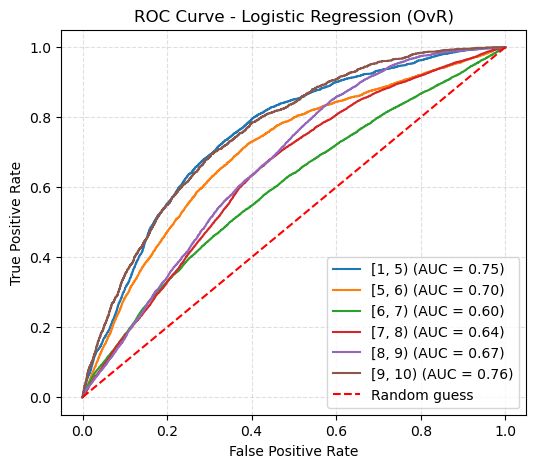
\includegraphics[width=\textwidth]{plotsss/log_roc_curves_rating.png} 
    \captionof{figure}{ROC curves for \texttt{rating\_class} (OvR)}
    \label{fig:log_roc_curves_rating} 
    \end{minipage}
\end{figure}





%-------------------------------------------------------------------------------
\subsection{Support Vector Machines}
\label{subsec:svm}

%-------------------------------------------------------------------------------
% titleType
%-------------------------------------------------------------------------------

We applied Support Vector Machines (SVM) to the \texttt{titleType} classification task.
Both linear and non-linear kernels were explored in order to evaluate how decision boundary complexity influences predictive performance.

The first experiment used a Linear SVM trained on the full dataset.  
A grid search with five-fold cross validation was carried out on the parameters 
$C \in \{0.01, 0.1, 1, 10, 100\}$ and $max\_iter \in \{1000, 5000, 10000\}$. 
The optimal configuration, with $C=100$ and $max\_iter=1000$, achieved a test accuracy of 0.81. 
While precision and recall were high for majority classes (\textit{movie}, \textit{short}, \textit{tvEpisode}), 
the classifier failed on \textit{tvSeries}, \textit{tvSpecial}, and \textit{video}, 
indicating that a linear decision boundary is insufficient for this problem.  

Non-linear kernels were then evaluated. 
A grid search was first performed on a stratified 10\% subset of the training set to efficiently explore a wide range of hyperparameters for each kernel, 
since a full search on the complete dataset would have been computationally prohibitive. 
All kernels were tested with $C$ ranging from 0.01 to 100 and $\gamma$ set to \texttt{scale} or \texttt{auto}.
For the polynomial kernel, the degree was varied between 2 and 4 and \texttt{coef0} set to 0 or 1.
For the sigmoid kernel, \texttt{coef0} was also explored at 0 and 1.
% $C$ was varied from 0.01 to 100 for all kernels.
% For the RBF kernel, $\gamma$ was set to \texttt{scale} or \texttt{auto}.
% The polynomial kernel was tested with degrees 2, 3 and 4, $\gamma$ as \texttt{scale} or \texttt{auto}, and \texttt{coef0} 0 or 1.
% The sigmoid kernel was explored with $\gamma$ \texttt{scale}/\texttt{auto} and \texttt{coef0} 0 or 1.

The best configuration for each kernel, reported in Table~\ref{tab:svm_results}, was then retrained on the full dataset and evaluated on the test set. 
Both RBF and polynomial kernels reached approximately 0.90 test accuracy, substantially outperforming the linear baseline and sigmoid. 
The RBF kernel was selected as the reference non-linear model due to slightly more stable results and improved recall on the under-represented classes.


% ROC curves were used to evaluate class separability 
% %(Figure~\ref{fig:roc_four}),
% showing excellent separation for majority classes, although minority categories remained problematic. 
% ???????????????????????????????????????????????????????????????
% ???????????????????????????????????????????????????????????????
% ???????????????????????????????????????????????????????????????

% \textcolor{red}{I will change the text and explain the figures better.}

To address class imbalance, the RBF kernel was retrained with \texttt{class\_weight=balanced}.
This model reached a slightly lower overall accuracy of 0.84, 
but recall for \textit{tvSpecial} and \textit{video} improved, providing a more equitable classification across categories.  
% Confusion matrices (Figure~\ref{fig:rbf_balanced_two}) 
% illustrate that \textit{tvSpecial} and \textit{video} ... 
The corresponding ROC curves (Figure~\ref{fig:rbf_balanced_two}b) show high separability for all classes, 
with AUC values of 0.99 for \textit{movie}, \textit{short}, and \textit{tvEpisode}, and 0.95 for \textit{tvSeries}, 
\textit{tvSpecial}, and \textit{video}, confirming that the balanced model achieves good discrimination 
for the minority categories too. 

Then an analysis of the support vectors was conducted.
In the unbalanced RBF, nearly all points of minority classes became support vectors, 
while in the balanced model the total number of support vectors increased but was more evenly distributed across classes, 
indicating a more complex but fairer decision function. 

Table~\ref{tab:svm_results} summarizes the main results, including the parameters used for each kernel and the corresponding test performance. 


\begin{table}[h]
\centering
\caption{Comparison of SVM models on the IMDb classification task.}
\label{tab:svm_results}
\begin{tabular}{lccc}
\hline
\textbf{Model} & \textbf{Best Params (main)} & \textbf{Test Accuracy} & \textbf{Macro F1-score} \\
\hline
Linear SVM & $C=100$, $max\_iter=1000$ & 0.81 & 0.45 \\
RBF kernel & $C=10$, $\gamma=\text{scale}$ & 0.90 & 0.64 \\
Polynomial kernel & $C=10$, degree=3, $\gamma=\text{auto}$ & 0.90 & 0.64 \\
Sigmoid kernel & $C=0.1$, $\gamma=\text{auto}$ & 0.65 & 0.36 \\
RBF (balanced) & $C=10$, $\gamma=\text{scale}$, balanced & 0.84 & 0.65 \\
\hline
\end{tabular}
\end{table}
    
% % --- First figure: four ROC curves side by side ---
% \begin{figure}[h]
%     \centering
%     \begin{subfigure}[b]{0.24\textwidth}
%         \centering
%         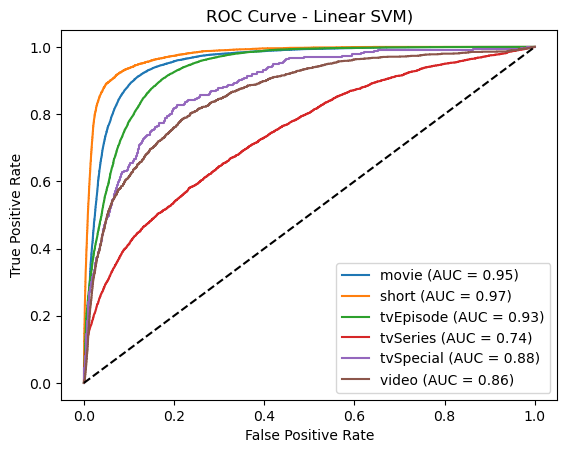
\includegraphics[width=\textwidth]{plotsss/roc_linear.png}
%         \caption{Linear SVM}
%         \label{fig:roc_linear}
%     \end{subfigure}
%     \begin{subfigure}[b]{0.24\textwidth}
%         \centering
%         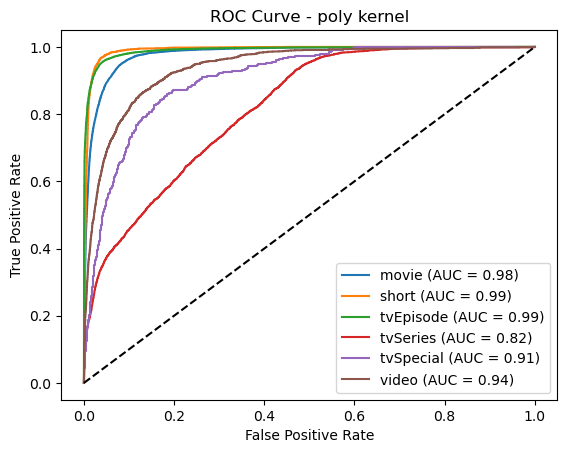
\includegraphics[width=\textwidth]{plotsss/roc_poly.png}
%         \caption{Polynomial kernel}
%         \label{fig:roc_poly}
%     \end{subfigure}
%     \begin{subfigure}[b]{0.24\textwidth}
%         \centering
%         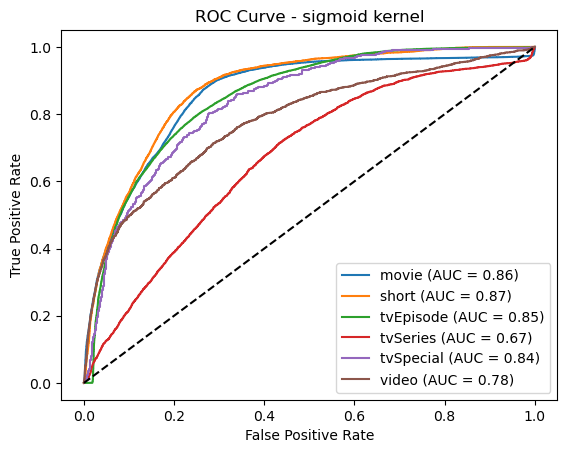
\includegraphics[width=\textwidth]{plotsss/roc_sigmoid.png}
%         \caption{Sigmoid kernel}
%         \label{fig:roc_sigmoid}
%     \end{subfigure}
%     \begin{subfigure}[b]{0.24\textwidth}
%         \centering
%         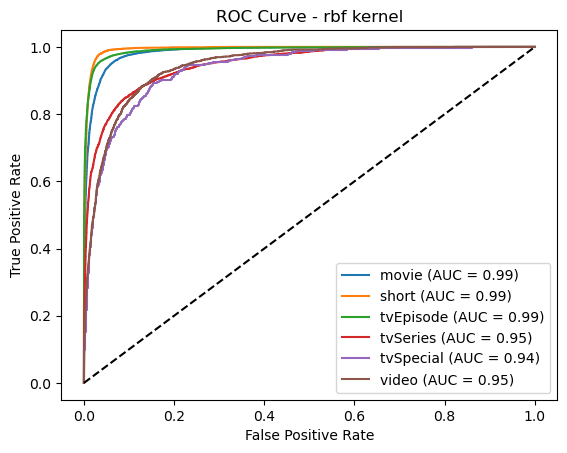
\includegraphics[width=\textwidth]{plotsss/roc_rbf.png}
%         \caption{RBF kernel}
%         \label{fig:roc_rbf}
%     \end{subfigure}
%     \caption{...}  
%     \label{fig:roc_four}
% \end{figure}

% --- Second figure: confusion matrix and ROC for RBF balanced ---
\begin{figure}[h]
    \centering
    \begin{subfigure}[b]{0.47\textwidth}
        \centering
        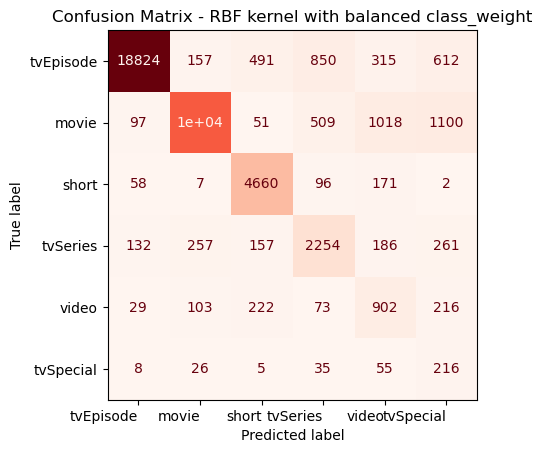
\includegraphics[width=\textwidth]{plotsss/new_cm_rbf_balanced.png}
        \caption{Confusion Matrix RBF balanced}
        \label{fig:cm_rbf_balanced}
    \end{subfigure}
    \begin{subfigure}[b]{0.43\textwidth}
        \centering
        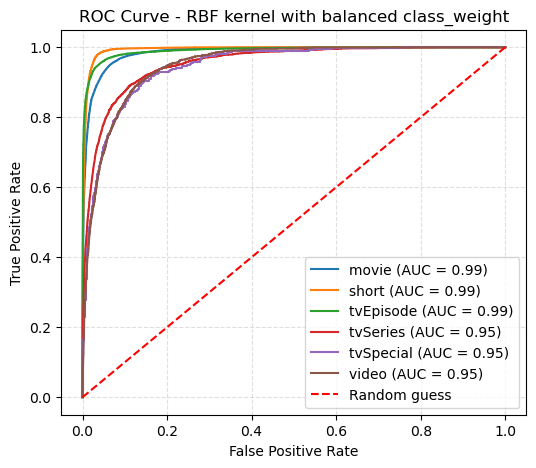
\includegraphics[width=\textwidth]{plotsss/new_roc_rbf_balanced.png}
        \caption{ROC RBF balanced}
        \label{fig:roc_rbf_balanced}
    \end{subfigure}
    \caption{Confusion Matrix and ROC Curve for the SVM (kernel rbf and balanced class weight) on the \texttt{titleType} classification task.}  
    \label{fig:rbf_balanced_two}
\end{figure}

% In conclusion, non-linear kernels were clearly superior to the linear SVM, 
% with RBF and polynomial achieving comparable accuracy. 
% The RBF kernel with balanced class weights provided the best compromise, 
% maintaining strong performance on majority classes while improving recognition of minority ones.

%-------------------------------------------------------------------------------
% rating
%-------------------------------------------------------------------------------

Support Vector Machines were applied to the \texttt{averageRating} classification task using the same kernels and hyperparameter search strategies as for \texttt{titleType}.
A Linear SVM achieved only 0.37 accuracy and a macro F1-score of 0.28, indicating that a linear decision boundary is inadequate.

Non-linear kernels were then explored. Both RBF and polynomial kernels reached similar test accuracy around 0.39, substantially outperforming the sigmoid kernel (0.28).
Due to slightly more stable results and better handling of minority categories, the RBF kernel was selected as the reference model.

To address class imbalance, the RBF model was retrained with \texttt{class\_weight=balanced}.
Overall accuracy decreased slightly to 0.29, but recall improved for the minority classes, particularly the extreme bins $[1,5)$ and $[9,10)$.
The classification report shows that the model captures a high proportion of extreme instances (recall 0.55 for $[1,5)$ and 0.63 for $[9,10)$), although precision is low (0.23 and 0.10, respectively), resulting in moderate F1-scores (0.33 and 0.18).
Intermediate bins are predicted with higher precision but lower recall, reflecting the difficulty of separating densely populated central categories.

ROC curves
%(Figure~\ref{fig:roc_rbf_balanced}) 
confirm this pattern: AUC is highest for the extremes ($[1,5)$: 0.79, $[9,10)$: 0.80) and lower for intermediate bins ($[6,7)$: 0.61, $[7,8)$: 0.65), indicating that the model distinguishes extreme ratings better than the mid-range values.

Overall, non-linear kernels improve performance over linear SVM, but the ordinal nature of \texttt{averageRating} and the strong class imbalance continue to challenge accurate prediction across all bins.

% \begin{figure}[h]
%     \centering
%     \includegraphics[width=0.5\textwidth]{plotsss/roc_rbf_balanced_rating.png}
%     \caption{ROC Curve for the SVM (kernel rbf and balanced class weight) on the \texttt{averageRating} classification task.}
%     \label{fig:roc_rbf_balanced}
% \end{figure}

%------------------------------
\subsection{Ensemble methods}
\begin{table}[H]
    \centering
    \begin{minipage}{0.55\textwidth}
        Boosting and Random Forest models were trained on the
        classification tasks, while being optimized via Stratified
        Randomized Search with 5-fold
        cross-validation over a predefined hyperparameter space.\\

        Table~\ref{tab:ensemble_param} shows the best
        hyperparameters found for Random Forest and AdaBoost on the
        \texttt{averageRating} task.\\

        For Random Forest, a relatively high maximum depth as well
        as low values for minimum samples per split and leaf
        indicate that the individual trees are quite complex.\\

        For AdaBoost, the base estimator is again characterized by
        high complexity. The learning rate is moderate, leading to
        reasonably fast learning.
    \end{minipage}
    \hfill
    \begin{minipage}{0.4\textwidth}
        \centering
        \begin{tabular}{lc}
        \hline
        % Best parameters found for Random Forest: {'class_weight': None, 'criterion': 'gini', 'max_depth': 19, 'max_features': 0.9137428250443735, 'min_samples_leaf': 6, 'min_samples_split': 2, 'n_estimators': 97}
        \multicolumn{2}{c}{\textbf{Random Forest}} \\
        \hline
        \texttt{n\_estimators} & 97 \\
        \texttt{max\_depth} & 19 \\
        \texttt{min\_samples\_split} & 2 \\
        \texttt{min\_samples\_leaf} & 6 \\
        \texttt{max\_features} & 0.91 \\
        \texttt{criterion} & gini \\
        \texttt{class\_weight} & \texttt{None} \\
        \hline
        \multicolumn{2}{c}{\textbf{AdaBoost}} \\
        \hline
        \texttt{n\_estimators} & 67 \\
        \texttt{learning\_rate} & 0.45 \\
        \texttt{estimator\_\_max\_depth} & 17 \\
        \texttt{estimator\_\_min\_samples\_split} & 7 \\
        \texttt{estimator\_\_min\_samples\_leaf} & 1 \\
        \hline
        \end{tabular}
        \caption{Hyperparameters found for ensemble models.}
        \label{tab:ensemble_param}
    \end{minipage}
\end{table}
The two models use a different number of estimators,
with Random Forest employing a larger ensemble.
This is likely due to the fact that Random Forest builds
trees independently, while AdaBoost adds weak learners
sequentially, focusing on correcting previous errors.

Another interesting aspect is the distribution of feature importances.
Both models assign most of the importance to the same set of features:
\begin{itemize}
    \item \texttt{ratingCount}
    \item \texttt{startYear}
    \item \texttt{runtimeMinutes}
    \item \texttt{deltaCredits}
\end{itemize}
Random Forest assigns about 50\% of the total importance to these
features, spreading it evenly among them.
AdaBoost assigns about 75\%, 41 of which is
attributed to \texttt{ratingCount} and \texttt{startYear}.



Table~\ref{tab:report_ensemble} summarizes the
classification report for both models.
Although the performances of the two models are similar,
Random Forest outperforms AdaBoost in all metrics but Macro-averaged
Precision. The weighted averaged metrics, here not reported,
also give the edge to Random Forest.

\begin{table}[H]
    \centering
    \begin{tabular}{lccccc}
    \hline
    \textbf{Model} & \textbf{Accuracy} & \textbf{Macro Precision} & \textbf{Macro Recall} & \textbf{Macro F1-score} \\
    \hline
    Random Forest & 0.45 & 0.47 & 0.35 & 0.37 \\
    AdaBoost & 0.43 & 0.49 & 0.33 & 0.35 \\
    \hline
    \end{tabular}
    \caption{Performances of the models on the \texttt{averageRating} classification task.}
    \label{tab:report_ensemble}
\end{table}
Performances of both models are limited, and the results show that
the different classes are not well separated. This can be observed
in Random Forest's confusion matrix in figure~\ref{fig:cm_rf}.
The matrix also shows that many of the misclassifications occur
within adjacent classes, which is expected given the ordinal
nature of the target variable.
In particular, a lot of confusion occurs between the most
represented classes, \texttt{[6,7)}, \texttt{[7,8)} and
\texttt{[8,9)}. This is likely due to the fact that these classes
cover a wide variety of titles that perform similarly in terms
of ratings. Additionally, as seen in graph~\ref{fig:rating_dist},
Many of the titles have ratings that fall close to the
boundaries between these classes, making it more difficult for the
model to distinguish between them.

\begin{figure}[H]
    \centering
    \begin{subfigure}[b]{0.44\textwidth}
        \centering
        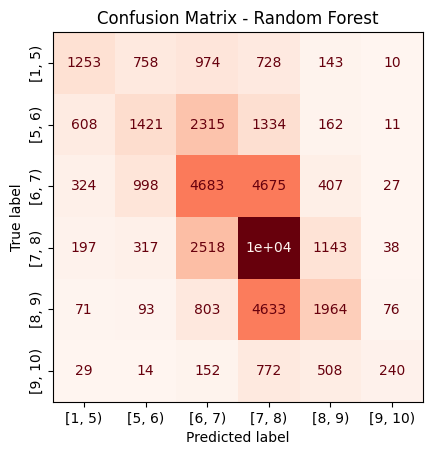
\includegraphics[width=\textwidth]{plotsss/conf_matr_rf_rating.png}
        \caption{Confusion Matrix - Random Forest}
        \label{fig:cm_rf}
    \end{subfigure}
    \hfill
    \begin{subfigure}[b]{0.52\textwidth}
        \centering
        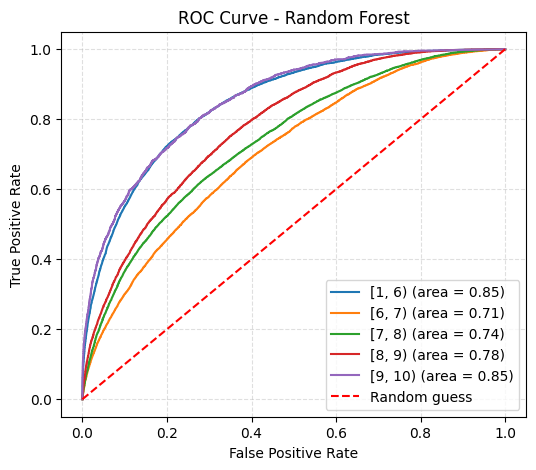
\includegraphics[width=\textwidth]{plotsss/roc_rf_rating.png}
        \caption{ROC Curve - Random Forest}
        \label{fig:roc_rating}
    \end{subfigure}
    \caption{Confusion matrix and ROC Curve for Random Forest on the \texttt{averageRating} classification task.}
    \label{fig:cm_roc_rating}
\end{figure}
Figure~\ref{fig:roc_rating} shows the ROC curve for AdaBoost.
% Min AUC: 70
AUCs are generally high, with the lowest ones being 0.70 and 0.72,
although these correspond to the highest-represented classes.
This suggests that the models are better at separating the
extreme classes, while the more frequent
intermediate ones are more difficult to distinguish.


%-------------------------------------------------------------------------------
% titleType ensemble
%-------------------------------------------------------------------------------


\begin{table}[H]
    \centering
    \begin{minipage}{0.55\textwidth}
        Table \ref{tab:ensemble_param_titletype} shows the best hyperparameter
        configurations found for Random Forest and AdaBoost on the
        \texttt{titleType} task.\\

        For Random Forest, the trees are quite deep and complex,
        with low minimum samples per split and leaf.\\

        For AdaBoost, the learning rate is very low, leading to
        slow, incremental learning.
        The base estimator is a decision tree with
        considerable depth and higher minimum samples per split and
        leaf than Random Forest's trees, indicating that each weak
        learner is slightly less complex.\\

        Again, the two models use a very different number of
        estimators, with Random Forest employing a much larger
        ensemble. For feature importances, both models assign
        over half of the importance to \texttt{runtimeMinutes},
        indicating a high dependence on this feature for
        classification.

    \end{minipage}
    \hfill
    \begin{minipage}{0.4\textwidth}
        \centering
        \begin{tabular}{lc}
        \hline
        \multicolumn{2}{c}{\textbf{Random Forest}} \\
        \hline
        \texttt{n\_estimators} & 42 \\
        \texttt{max\_depth} & 19 \\
        \texttt{min\_samples\_split} & 4 \\
        \texttt{min\_samples\_leaf} & 3 \\
        \texttt{max\_features} & 0.74 \\
        \texttt{criterion} & gini \\
        \texttt{class\_weight} & \texttt{None} \\
        \hline
        \multicolumn{2}{c}{\textbf{AdaBoost}} \\
        \hline
        \texttt{n\_estimators} & 11 \\
        \texttt{learning\_rate} & 0.03 \\
        \texttt{estimator\_\_max\_depth} & 14 \\
        \texttt{estimator\_\_min\_samples\_split} & 18 \\
        \texttt{estimator\_\_min\_samples\_leaf} & 10 \\
        \hline
        \end{tabular}
        \caption{Hyperparameter search space for ensemble models.}
        \label{tab:ensemble_param_titletype}
    \end{minipage}
    
\end{table}

Table~\ref{tab:classification_report} summarizes the classification report for both models.
\begin{table}[H]
    \centering
    \begin{tabular}{lccccc}
    \hline
    \textbf{Model} & \textbf{Accuracy} & \textbf{Macro Precision} & \textbf{Macro Recall} & \textbf{Macro F1-score} \\
    \hline
    Random Forest & 0.92 & 0.84 & 0.71 & 0.75 \\
    AdaBoost & 0.92 & 0.81 & 0.70 & 0.73 \\
    \hline
    \end{tabular}
    \caption{Performances of the models on the \texttt{titleType} classification task.}
    \label{tab:classification_report}
\end{table}


Figures~\ref{fig:cm_rf_titletype} shows the confusion matrix
for Random Forest.
Consistently good performances can be observed across the most
represented classes. \texttt{video} and \texttt{tvSpecial} are the
classes that cause the most problems, since they are often
misclassified as the more frequent classes. The class \texttt{movie}
attracts most of these misclassifications, likely due to
similar durations of the products in these categories.
Likely due to the same reason, \texttt{video} is also often
misclassified as \texttt{short}.\\

\begin{figure}[H]
    \centering
    \begin{subfigure}[b]{0.47\textwidth}
        \centering
        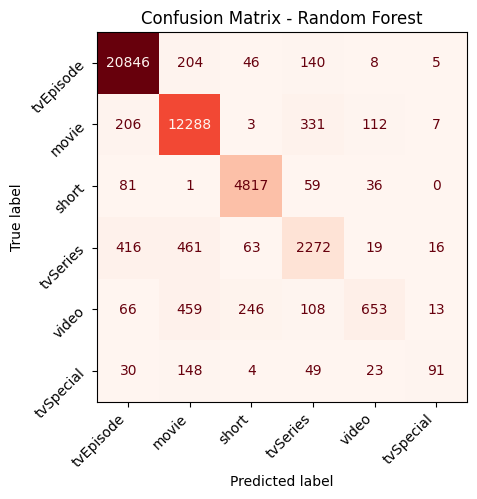
\includegraphics[width=\textwidth]{plotsss/conf_matr_rf_titletype}
        \caption{Confusion Matrix - Random Forest}
        \label{fig:cm_rf_titletype}
    \end{subfigure}
    \hfill
    \begin{subfigure}[b]{0.50\textwidth}
        \centering
        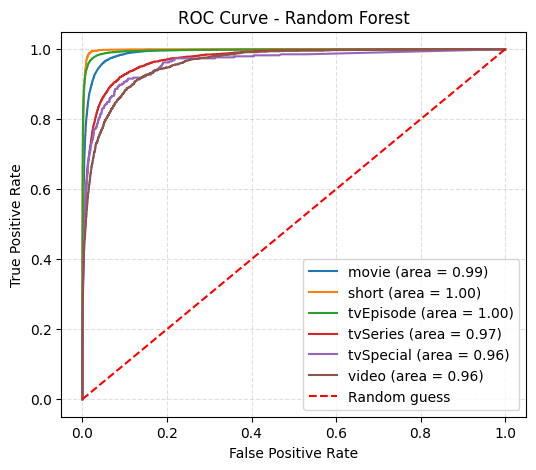
\includegraphics[width=\textwidth]{plotsss/roc_rf_titletype}
        \caption{ROC Curve - Random Forest}
        \label{fig:roc_rf}
    \end{subfigure}
    \caption{Confusion matrix and ROC Curve for Random Forest on the \texttt{titleType} classification task.}
    \label{fig:cm_comparison}
\end{figure}

The ROC curve shows high AUCs for all classes, with the lowest ones
being for the aformentioned less represented classes, both
achieving 0.96. This indicates that the model is very good at
maintaining a low false positive rate for these, while
correctly identifying the more represented classes.


\subsection{Neural Networks}

For both classification tasks, a feedforward neural network was
implemented.\\

% Input(shape=(X_train.shape[1],)),
    % Dense(8, activation='relu'),
    % Dense(16, activation='relu'),
    % Dense(32, activation='relu'),
    % Dense(64, activation='relu'),
    % Dense(32, activation='relu'),
    % Dropout(0.2),
    % Dense(16, activation='relu'),
    % Dense(8, activation='relu'),
    % Dense(6, activation='softmax')
For the \texttt{averageRating} task, the architecture consists of
an input layer, six hidden layers with ReLU activation, forming a
diamond shape (increasing and then decreasing number of neurons),
a dropout layer (rate 0.2) to prevent overfitting, and an output
layer with softmax activation for multi-class classification.\\
The model was compiled with the Adam optimizer, categorical
cross-entropy loss, and accuracy as the evaluation metric.
No early stopping was used, in order to observe the full
training dynamics. Training was set to last for 500 epochs, with a
batch size of 64 and a validation split of 20\%.


Figures~\ref{fig:loss_nn_rating} and~\ref{fig:accuracy_nn_rating}
show the training and validation loss and accuracy over epochs.
The training loss shows a steady decrease, while the validation loss
stops improving after around 100 to 150 epochs.
A similar trend is observed in the accuracy plot, although the
end of the the rise can be found after around 200 epochs.
Neither graph shows particular signs of overfitting, but
the stagnation of the validation metrics suggests that the model
could benefit from further regularization.
Experiments were made with different dropout rates and configurations,
as well as different training batch sizes and learning rates,
in an attempt to improve generalizaiton, but this remained the
best configuration found.\\

\begin{figure}[H]
    \centering
    \begin{subfigure}[b]{0.48\textwidth}
        \centering
        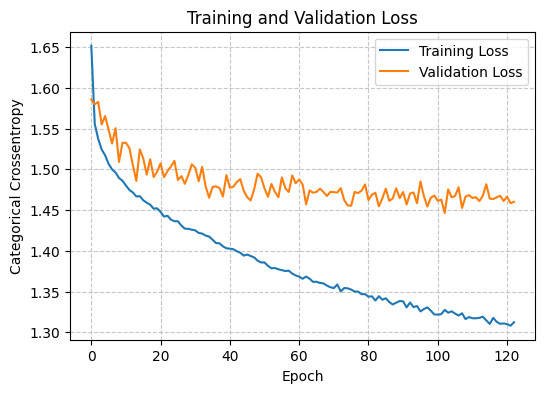
\includegraphics[width=\textwidth]{plotsss/loss_rating.png}
        \caption{Loss - Neural Network}
        \label{fig:loss_nn_rating}
    \end{subfigure}
    \hfill
    \begin{subfigure}[b]{0.48\textwidth}
        \centering
        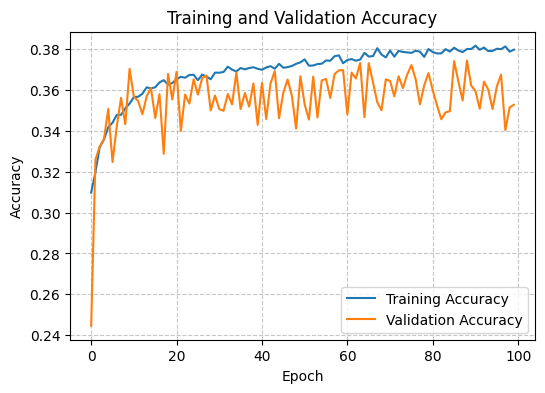
\includegraphics[width=\textwidth]{plotsss/accuracy_rating.png}
        \caption{Accuracy - Neural Network}
        \label{fig:accuracy_nn_rating}
    \end{subfigure}
    \caption{Training and validation loss and accuracy for the neural network on the \texttt{averageRating} classification task.}
    \label{fig:nn_performance_rating}
\end{figure}

\begin{figure}[H]
    \centering
    \begin{subfigure}[b]{0.45\textwidth}
        \centering
        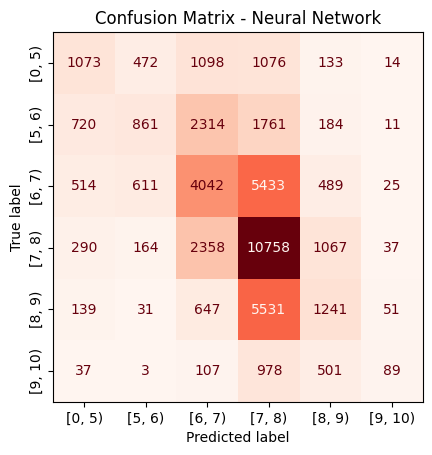
\includegraphics[width=\textwidth]{plotsss/cm_nn_rating.png}
        \caption{Confusion Matrix - Neural Network}
        \label{fig:cm_nn_rating}
    \end{subfigure}
    \hfill
    \begin{subfigure}[b]{0.53\textwidth}
        \centering
        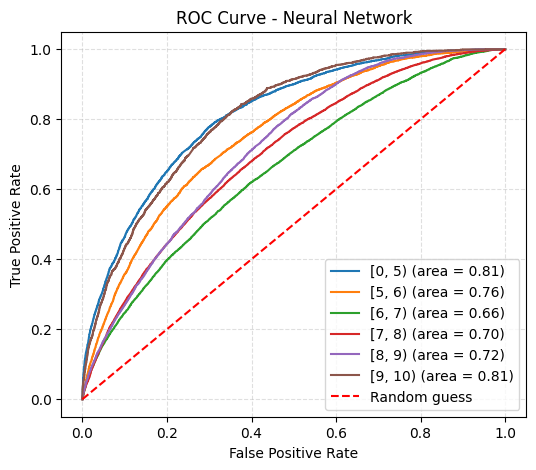
\includegraphics[width=\textwidth]{plotsss/roc_nn_rating.png}
        \caption{ROC Curve - Neural Network}
        \label{fig:roc_nn_rating}
    \end{subfigure}
    \caption{Confusion Matrix and ROC Curve for the Neural Network on the \texttt{averageRating} classification task.}
    \label{fig:cm_roc_nn}
\end{figure}


\begin{table}
    \centering
    \begin{tabular}{lccc}
    \hline
     & \textbf{Precision} & \textbf{Recall} & \textbf{F1-score}\\
    \hline
    \textbf{Macro avg}   & 0.39 & 0.29 & 0.29 \\
    \textbf{Weighted avg}& 0.39 & 0.40 & 0.36 \\
    \hline
    \textbf{Accuracy}    & & & 0.40 \\
    \hline
    \end{tabular}
    \caption{Classification performances for the neural network on the \texttt{averageRating} classification task.}
    \label{tab:nn_report_rating}
\end{table}


% -------------------------------------------------------------------------------
% titletype task
% -------------------------------------------------------------------------------


\begin{figure}[H]
    \centering
    \begin{subfigure}[b]{0.48\textwidth}
        \centering
        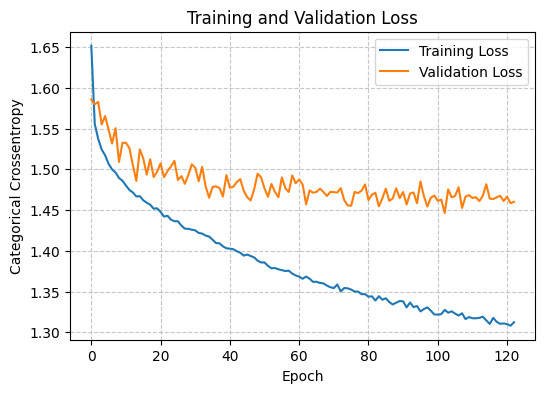
\includegraphics[width=\textwidth]{plotsss/loss_titletype.png}
        \caption{Loss - Neural Network}
        \label{fig:loss_nn_titletype}
    \end{subfigure}
    \hfill
    \begin{subfigure}[b]{0.48\textwidth}
        \centering
        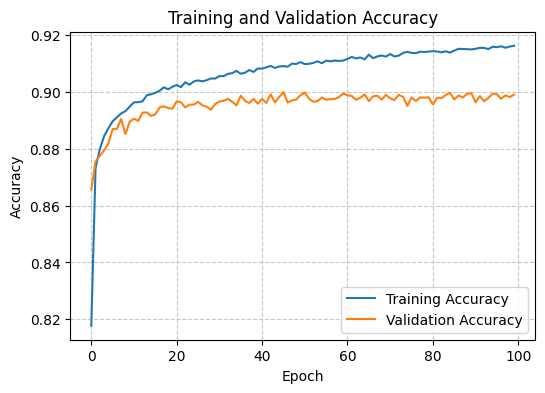
\includegraphics[width=\textwidth]{plotsss/accuracy_titletype.png}
        \caption{Accuracy - Neural Network}
        \label{fig:accuracy_nn_titletype}
    \end{subfigure}
    \caption{Training and validation loss and accuracy for the neural network on the \texttt{titleType} classification task.}
    \label{fig:nn_performance_titletype}
\end{figure}

% conf matrix and roc titletype

\begin{figure}[H]
    \centering
    \begin{subfigure}[b]{0.47\textwidth}
        \centering
        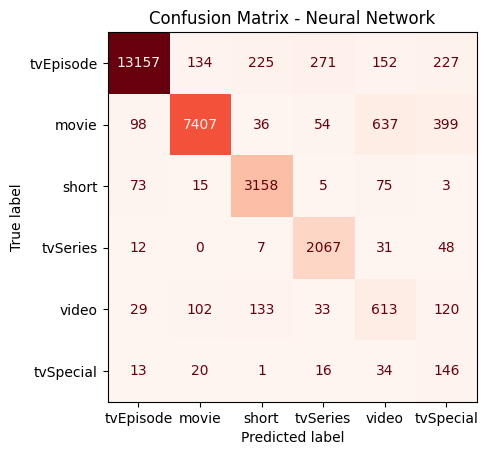
\includegraphics[width=\textwidth]{plotsss/cm_nn_titletype.png}
        \caption{Confusion Matrix - Neural Network}
        \label{fig:cm_nn_titletype}
    \end{subfigure}
    \hfill
    \begin{subfigure}[b]{0.50\textwidth}
        \centering
        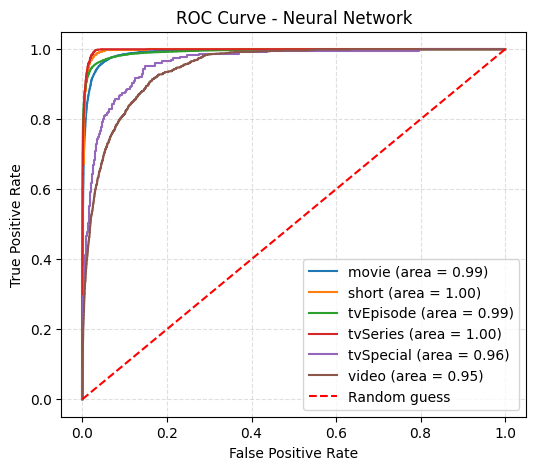
\includegraphics[width=\textwidth]{plotsss/roc_nn_titletype.png}
        \caption{ROC Curve - Neural Network}
        \label{fig:roc_nn_titletype}
    \end{subfigure}
    \caption{Confusion Matrix and ROC Curve for the Neural Network on the \texttt{titleType} classification task.}
    \label{fig:cm_nn_titletype}
\end{figure}

\subsection{Gradient Boosting Machines}
Next, we applied a \texttt{Gradient Boosting Machine (GBM)} to evaluate its ability to classify the \texttt{titleType} and \texttt{rating\_bin} variable. 
\texttt{GBM} is an ensemble method that builds a series of decision trees sequentially, where each tree attempts to correct 
the errors of its predecessor. Unlike \texttt{Random Forest}, which builds trees independently and averages their predictions, 
\texttt{GBM} focuses on minimizing the loss function through gradient descent, making it highly adaptive to complex patterns in the data.
The baseline accuracy to predict \texttt{titleType} was found out to be 0.94, while for \texttt{rating\_bin} it was 0.40.
For both tasks, we sampled the data to 10\% of the training set to perform hyperparameter tuning, 
due to the high computational cost of training GBM models on large datasets.
The hyperparameter tuning was performed using \texttt{RandomizedSearchCV} with 5-fold stratified cross-validation.
Table \ref{tab:GBM_param} shows the best parameters found for the \texttt{titleType} and \texttt{rating\_bin}.
\begin{table}[H]
    \centering
    \begin{minipage}{0.4\textwidth}
        \centering
        \begin{tabular}{lc}
        \hline
        \multicolumn{2}{c}{\textbf{titleType}} \\
        \hline
        \texttt{subsample} & 0.8 \\
        \texttt{n\_estimators} & 500 \\
        \texttt{max\_depth} & 6 \\
        \texttt{min\_samples\_split} & 10 \\
        \texttt{min\_samples\_leaf} & 1 \\
        \texttt{max\_features} & None \\
        \texttt{learning\_rate} & 0.1 \\
        \hline
        \multicolumn{2}{c}{\textbf{rating\_bin}} \\
        \hline
        \texttt{subsample} & 0.6 \\
        \texttt{n\_estimators} & 400 \\
        \texttt{max\_depth} & 5 \\
        \texttt{min\_samples\_split} & 10 \\
        \texttt{min\_samples\_leaf} & 2 \\
        \texttt{max\_features} & sqrt \\
        \texttt{learning\_rate} & 0.05 \\
        \hline
        \end{tabular}
        \caption{Hyperparameter search space for GBM.}
        \label{tab:GBM_param}
    \end{minipage}
    
\end{table}

% \begin{center}
%     'subsample': 0.8, 'n\_estimators': 500, 'min\_samples\_split': 10, 'min\_samples\_leaf': 1, 'max\_features': None, 'max\_depth': 6, 'learning\_rate': 0.1
% \end{center}
% The best parameters found for the \texttt{rating\_bin} task were:
% \begin{center}
%     'subsample': 0.6, 'n\_estimators': 400, 'min\_samples\_split': 10, 'min\_samples\_leaf': 2, 'max\_features': 'sqrt', 'max\_depth': 5, 'learning\_rate': 0.05
% \end{center}

\begin{figure}[ht]
    \centering
    \begin{minipage}{0.45\textwidth} 
    \centering
    \captionof{table}{Classification report for \texttt{titleType}}
    \label{tab:GBM_report_t}
    \small 
    \begin{tabular}{lccc}
    \hline
    \textbf{Class} & \textbf{Precision} & \textbf{Recall} & \textbf{F1-score}\\
    \hline
    tvEpisode  & 0.94 & 0.97 & 0.96  \\
    movie      & 0.95 & 0.98 & 0.97  \\
    short      & 0.98 & 0.98 & 0.98  \\
    tvSeries   & 0.94 & 0.97 & 0.96  \\
    video      & 0.77 & 0.45 & 0.57  \\
    tvSpecial  & 0.79 & 0.55 & 0.65  \\
    \hline
    \textbf{Accuracy}    & \multicolumn{3}{c}{0.96} \\
    \textbf{Macro avg}   & 0.90 & 0.82 & 0.85  \\
    \textbf{Weighted avg}& 0.96 & 0.96 & 0.96  \\
    \hline
    \end{tabular}
    \end{minipage}
    \hfill
    \begin{minipage}{0.4\textwidth} 
    \centering
    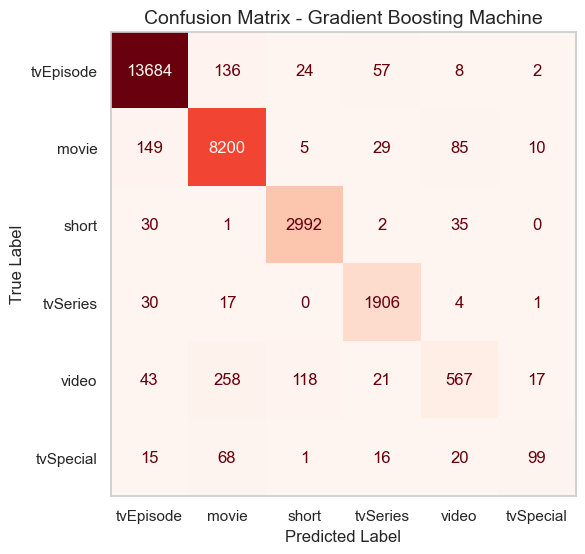
\includegraphics[width=\textwidth]{plotsss/GBM_confusion_title.png} 
    \captionof{figure}{Confusion Gradient Boosting Machine}
    \label{fig:GBM_confusion_title} 
    \end{minipage}
    \begin{minipage}{0.4\textwidth} 
    \centering
    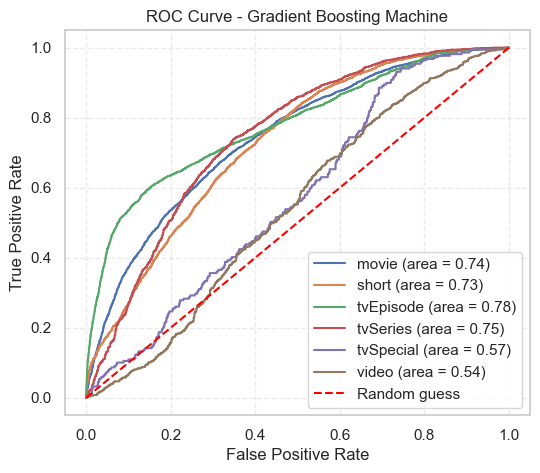
\includegraphics[width=\textwidth]{plotsss/GBM_ROC_title.png} 
    \captionof{figure}{ROC Gradient Boosting Machine}
    \label{fig:GBM_ROC_title} 
    \end{minipage}

    \end{figure}

From the table \ref{tab:GBM_report_t}, we can see that GBM performs very well on the \texttt{titleType} task, achieving an accuracy of 0.96.
The confusion matrix (Figure~\ref{fig:GBM_confusion_title}) shows that the model is able to correctly classify most of the classes, 
with only a few misclassifications recorded for the less represented classes \texttt{video} and \texttt{tvSpecial}.
The ROC curves (Figure~\ref{fig:GBM_ROC_title}) also show high AUC values for all classes, 
indicating that the model is able to separate the classes well.
The differences in ROC curve suggest that the model is more effective at distinguishing structured and well-documented 
categories such as \textit{tvEpisode}, \textit{tvSeries}, and \textit{movie}, 
To further investigate, we examined feature importance and found that \texttt{runtimeMinutes}, \texttt{numRegions}, 
and \texttt{directorCredits} were among the most influential features. 
Titles with longer runtimes and broader regional distribution were more likely to be classified as \textit{movies} or \textit{tvSeries}, 
while shorter or regionally limited titles tended to fall into categories like \textit{short} or \textit{video}. 
The number of director credits also served as a proxy for production quality and documentation, 
helping the model differentiate between professionally produced content and less formal formats. 
Interestingly, the \textit{Europe} feature emerged as a strong predictor, 
possibly due to cultural or market-specific trends in title type distribution. 


\begin{figure}[ht]
    \centering
    \begin{minipage}{0.45\textwidth} 
    \centering
    \captionof{table}{Classification report for \texttt{titleType}}
    \label{tab:GBM_report_r}
    \small 
    \begin{tabular}{lccc}
    \hline
    \textbf{Class} & \textbf{Precision} & \textbf{Recall} & \textbf{F1-score}\\
    \hline
    0  & 0.49 & 0.38 & 0.43  \\
    1      & 0.37 & 0.26 & 0.31  \\
    2      & 0.41 & 0.39 & 0.40  \\
    3   & 0.47 & 0.67 & 0.56  \\
    4      & 0.43 & 0.30 & 0.35  \\
    5  & 0.44 & 0.22 & 0.29  \\
    \hline
    \textbf{Accuracy}    & \multicolumn{3}{c}{0.44} \\
    \textbf{Macro avg}   & 0.44 & 0.37 & 0.39  \\
    \textbf{Weighted avg}& 0.44 & 0.44 & 0.43  \\
    \hline
    \end{tabular}
    \end{minipage}
    \hfill
    \begin{minipage}{0.4\textwidth} 
    \centering
    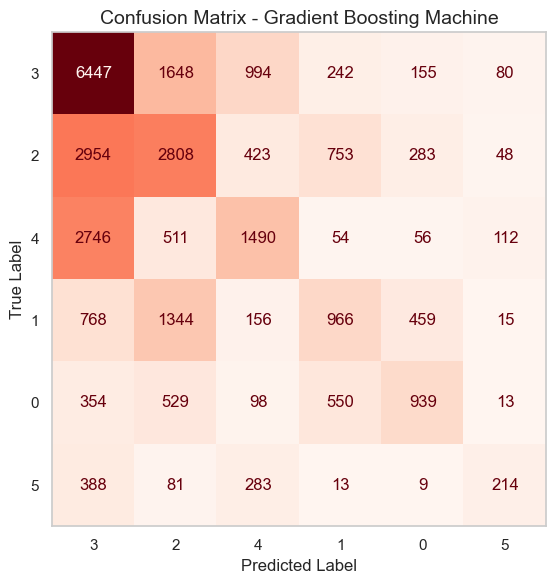
\includegraphics[width=\textwidth]{plotsss/GBM_confusion_rating.png} 
    \captionof{figure}{Confusion Matrix Gradient Boosting Machine}
    \label{fig:GBM_confusion_rating} 
    \end{minipage}
    \begin{minipage}{0.4\textwidth} 
    \centering
    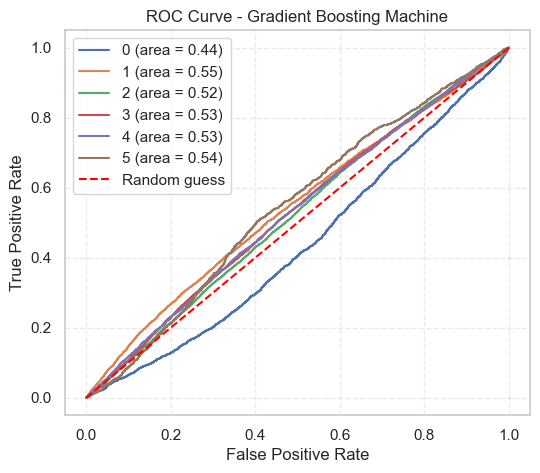
\includegraphics[width=\textwidth]{plotsss/GBM_ROC_rating.png} 
    \captionof{figure}{ROC Gradient Boosting Machine}
    \label{fig:GBM_ROC_rating} 
    \end{minipage}

    \end{figure}

From the table \ref{tab:GBM_report_r}, it is evident that the Gradient Boosting Machine performs moderately on the 
\texttt{rating\_bin} classification task, achieving an overall accuracy of 0.44. While this is less than 50\%, 
considering that the task involves six classes, the model exceeds the baseline accuracy of 1/6, indicating that it is 
capturing some underlying patterns in the data. Examination of the confusion matrix (Figure~\ref{fig:GBM_confusion_rating}) 
reveals that the model correctly classifies rating class 3 more reliably than others, while classes 2 and 4 are often misclassified 
as 3, and classes 0, 1, and 5 exhibit similar tendencies. A noteworthy observation is that misclassifications tend to 
occur between neighboring classes, whereas classes that are further apart, such as 0 and 5, are rarely confused. 
This suggests that the model is not producing random predictions, but rather that the proximity and overlap of 
class distributions present inherent challenges in distinguishing closely spaced ratings.

The ROC curves (Figure~\ref{fig:GBM_ROC_rating}) reinforce this observation, 
showing relatively low AUC values of approximately 0.54 for all classes, which indicates limited 
separability among the rating bins. Compared to tasks such as \textit{titleType}, the model struggles to distinguish \textit{rating\_bin}, 
likely due to the continuous and overlapping nature of ratings as opposed to the more discrete and structured categories of title types. 
Feature importance analysis provides additional insight: \textit{ratingCount} emerges as the strongest predictor, 
which is intuitive since titles with higher ratings are more likely to be correctly classified. 
\textit{StartYear} appears influential, potentially reflecting temporal trends in ratings, 
while \textit{runtimeMinutes} indicates that longer titles tend to receive higher ratings. 
Other features such as \textit{totalCredits}, \textit{castNumber}, \textit{totalMedia}, and \textit{tvEpisode} also contribute significantly, 
with \textit{tvEpisode} being more impactful than other TV formats like \textit{tvMiniseries}, \textit{tvSpecial}, or \textit{tvShort}, 
possibly due to greater representation in the dataset.
Overall, the results suggest that while the model captures broad patterns such as the tendency for longer or more regionally distributed titles to receive higher ratings, 
it struggles with fine-grained distinctions between closely spaced rating bins. 



\subsection{Model Comparison}

\subsection{Explainable AI}
To better understand the predictions made by our Neural Network model, we employed \texttt{LIME} Local Interpretable Model-agnostic Explanations 
to provide local explanations for individual predictions.
LIME works by perturbing the input data around a specific instance and 
observing how the model's predictions change. 
This allows us to identify which features are most influential for that particular prediction.
For our analysis, we selected the first instance from the test set of both classification tasks: \texttt{titleType} and \texttt{averageRating}.
We then used LIME to generate explanations for the model's predictions on these instances.

\subsubsection{titleType}

 
\begin{figure}[htbp]
    \centering
    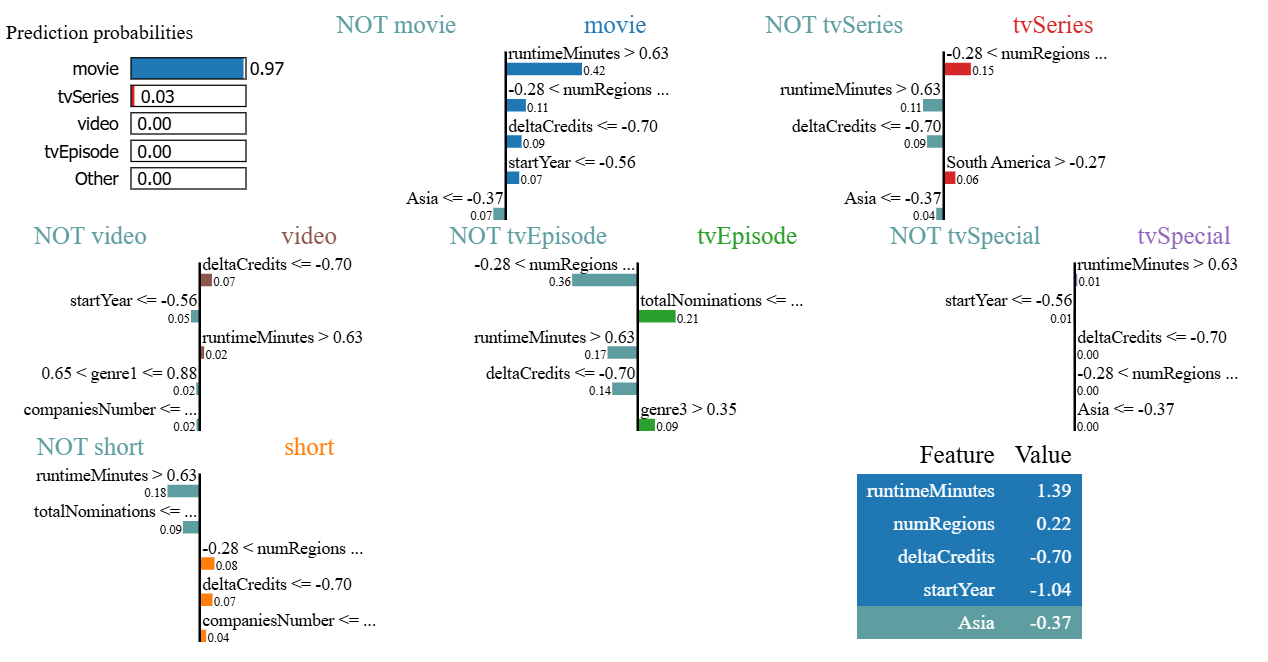
\includegraphics[width=\linewidth]{plotsss/Lime_title.png}
    \caption{LIME explanation for the \texttt{titleType} prediction of instance 0 in the test set.}
    \label{fig:LIME_title}
\end{figure}
Figure~\ref{fig:LIME_title} shows the LIME explanation for the \texttt{titleType} prediction of instance 0. We only show the top 5 features for clarity.
The model assigns a high probability of 0.97 to the class \textit{movie}, with all other classes receiving negligible scores. 
This strong confidence is supported by the decision rules extracted from the local surrogate model, which highlight 
the most influential features contributing to the classification. 
The top features include \texttt{runtimeMinutes}, \texttt{numRegions}, \texttt{deltaCredits}, and \texttt{startYear}, 
each evaluated against specific thresholds. For instance, the value of \texttt{runtimeMinutes} is 1.39 (standardized), 
which exceeds the threshold used to exclude categories such as \textit{short} and \textit{tvEpisode}, 
both of which typically have shorter durations. Similarly, the low value of \texttt{numRegions} (0.28) and \texttt{deltaCredits} (0.01) 
helps eliminate classes like \textit{video} and \textit{tvSpecial}, which often have limited regional distribution and sparse production metadata. 
The standardized \texttt{startYear} value of $-1.04$ suggests an older release date, 
which may align more closely with traditional \textit{movie} formats than episodic or special content. 
The decision paths shown in the visualization reinforce the model's reasoning by systematically ruling out 
alternative classes through feature-based logic. Notably, the absence of branching toward competing categories 
like \textit{tvSeries} or \textit{video} indicates that the feature profile of this instance is highly aligned with the 
learned representation of a \textit{movie}. \\

Figure~\ref{fig:title_coeff} presents the top five features contributing to the model's prediction for a specific instance '0'
in the \texttt{titleType} classification task. The feature \texttt{runtimeMinutes > 0.63} has the highest positive contribution of 0.4208, 
indicating that longer runtimes strongly support the classification decision, likely favoring categories such as \textit{movie} or \textit{tvSeries}. 
The condition \texttt{-0.28 < numRegions $\leq$ 0.57} contributes 0.1110, suggesting that moderate regional distribution adds further support 
to the predicted class, possibly reflecting titles with limited but non-trivial geographic reach. 
The feature \texttt{deltaCredits $\leq$ -0.70}, with a contribution of 0.0875, implies that a low difference between director and writer credits 
may signal a more streamlined or unified production, which is often characteristic of traditional movie formats. 
The condition \texttt{startYear $\leq$ -0.56} contributes 0.0744, indicating that older titles are more likely to belong to certain categories, 
perhaps due to historical production norms or metadata completeness. Interestingly, the feature \texttt{Asia $\leq$ -0.37} 
has a negative contribution of $-0.0688$, suggesting that limited association with the Asian region reduces the likelihood of 
certain title types, possibly reflecting regional content trends or distribution biases. Collectively, these contributions reveal how the model 
leverages both structural and geographic metadata to make confident predictions, and they underscore the interpretability of the decision-making process 
through localized feature analysis.

\begin{figure}
    \centering
    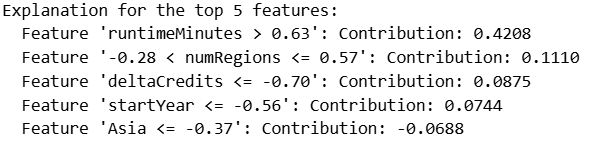
\includegraphics[width=0.7\textwidth]{plotsss/title_coeff.png}
    \caption{Contribution of top 5 features}
    \label{fig:title_coeff}
\end{figure}

\subsubsection{averageRating}

\begin{figure}[htbp]
    \centering
    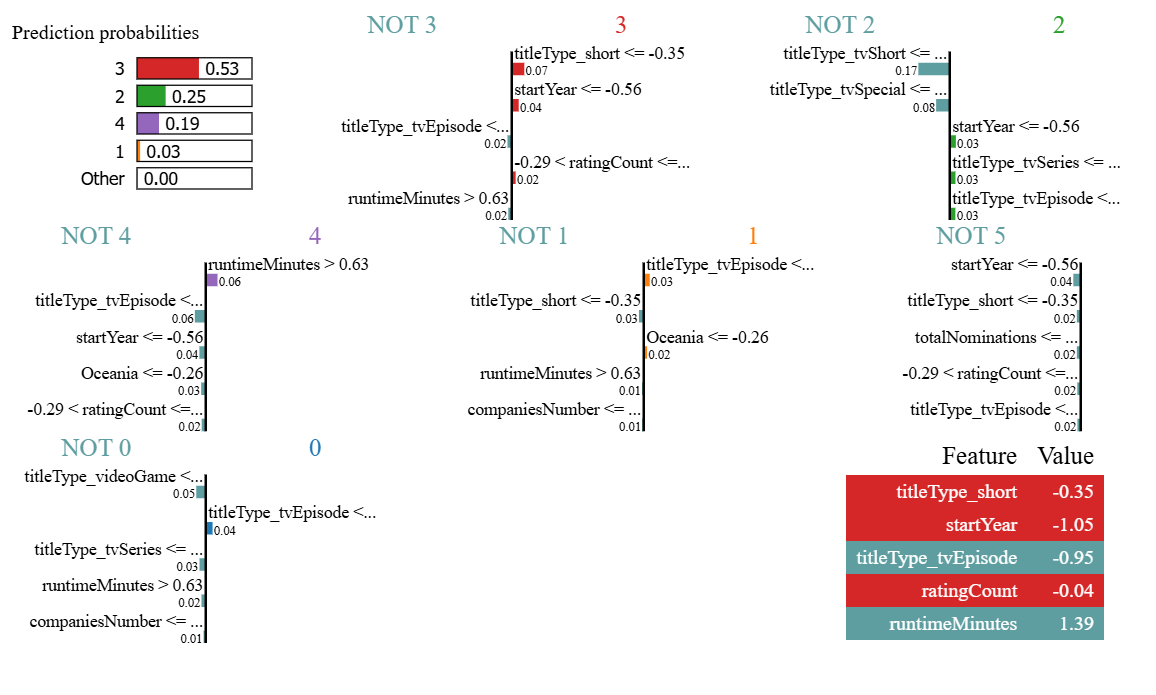
\includegraphics[width=\linewidth]{plotsss/Lime_rating.png}
    \caption{LIME explanation for the \texttt{rating\_class} prediction of instance 0 in the test set.}
    \label{fig:LIME_rating}
\end{figure}

Figure~\ref{fig:LIME_rating} presents the LIME explanation for the \texttt{rating\_class} 
prediction of instance 0 in the test set, generated from a sequential neural network model. 
The predicted class is 0, with a confidence of 53\%, followed by class 1 (25\%), class 2 (13\%), and class 3 (9\%), 
indicating a moderate level of uncertainty but a clear preference toward the lowest rating bin. 
For this instance, \texttt{titleType\_short = 0.43} and \texttt{titleType\_tvEpisode = 0.5} suggest the content 
is neither a short nor a TV episode, which may steer the model away from mid-range rating bins typically 
associated with episodic or short-form content. The value \texttt{startYear = -1.05} indicates an older release, 
which often correlates with lower ratings due to outdated production standards or limited contemporary relevance. 
Additionally, \texttt{ratingCount = -0.25} reflects low audience engagement, reinforcing the likelihood of a 
lower rating bin. Interestingly, \texttt{runtimeMinutes = 1.39} suggests a longer duration, which might typically 
support higher ratings, but in this context, it appears insufficient to offset the negative influence of other 
features. The surrogate explanation reveals how the neural network integrates temporal, structural, and 
popularity-related metadata to arrive at its prediction, and it highlights the nuanced interplay 
between feature thresholds and class probabilities in a locally interpretable manner.

\begin{figure}
    \centering
    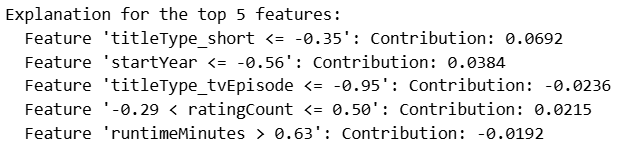
\includegraphics[width=0.7\textwidth]{plotsss/rating_coeff.png}
    \caption{Contribution of top 5 features}
    \label{fig:rating_coeff}
\end{figure}


Figure~\ref{fig:rating_coeff} illustrates the top five features influencing the model's 
prediction for the \texttt{rating\_bin} classification. The feature \texttt{titleType\_short $\leq$ -0.35} 
contributes positively with a value of 0.0692, suggesting that titles categorized as "short" are more likely to fall into a 
specific rating bin, possibly due to their niche appeal or limited exposure. The feature \texttt{startYear $\leq$ -0.56} 
adds a contribution of 0.0384,potentially reflecting historical rating standards or audience expectations.
Conversely, the feature \texttt{titleType\_tvEpisode $\leq$ -0.95} has a negative contribution of $-0.0236$, implying that the 
absence or low presence of TV episodes reduces the likelihood of the predicted rating bin, possibly due to episodic 
content receiving more polarized ratings. The condition \texttt{-0.29 < ratingCount $\leq$ 0.50} contributes 0.0215, 
suggesting that moderate rating counts slightly support the classification, likely reflecting a balance between popularity 
and niche interest. Lastly, \texttt{runtimeMinutes > 0.63} contributes negatively with $-0.0192$, indicating that 
longer runtimes may detract from the predicted rating bin, perhaps due to pacing issues or audience fatigue.
The model appears to weigh structural metadata (e.g., title type, runtime) alongside temporal 
and popularity indicators to infer rating categories. Overall, The model's interpretability lies in its transparent structure, 
allowing us to trace how each feature contributes to the final classification. 
This is particularly valuable for validating predictions and identifying potential biases in the training data.